\documentclass[sigconf]{acmart}
\settopmatter{printacmref=false} % Removes citation information below abstract
%\renewcommand\footnotetextcopyrightpermission[1]{} % removes footnote with conference information in first column
\pagestyle{plain} % removes running headers
\pagestyle{empty}

\usepackage{array}
\usepackage{graphicx}
\usepackage{clrscode}
\usepackage{balance}
\usepackage{subfigure}
\usepackage{multirow}
\usepackage{float}
\usepackage{color}
\usepackage{soul}
\usepackage{mdframed}
\usepackage{amsopn}
\usepackage{mathrsfs}
\usepackage{mathtools}
\usepackage{amsmath}
\usepackage{arydshln}
\usepackage{hyperref}
\usepackage{multicol}
\usepackage{blkarray}
\usepackage{enumerate}
\usepackage{courier}
\usepackage{rotating}
\usepackage{booktabs}
\usepackage{diagbox}
\usepackage{fancybox}
\usepackage{minibox}
\usepackage{cases}
\usepackage[lined,boxruled,commentsnumbered,linesnumbered]{algorithm2e}

\newcommand{\ylcomment}[1]{\textcolor{blue}{[#1---yl]}}

\DeclareRobustCommand{\hlblue}[1]{{\sethlcolor{blue}\hl{#1}}}
\DeclareRobustCommand{\hlgreen}[1]{{\sethlcolor{green}\hl{#1}}}
\DeclareRobustCommand{\hlred}[1]{{\sethlcolor{red}\hl{#1}}}

\newcommand{\argmin}{\operatornamewithlimits{argmin}}
\newcommand{\argmax}{\operatornamewithlimits{argmax}}
\newcommand{\minimize}{\operatornamewithlimits{minimize}}
\newcommand{\maximize}{\operatornamewithlimits{maximize}}
\newcommand{\random}{\operatornamewithlimits{random}}
\newcommand{\suchthat}{\operatornamewithlimits{s.t.}}
\newcommand{\rank}{\operatornamewithlimits{rank}}
\newcommand{\trace}{\operatorname{tr}}
\newcommand{\vectorize}{\operatornamewithlimits{vec}}
\newcommand{\diag}{\operatornamewithlimits{diag}}
\newcommand{\bdf}{\operatornamewithlimits{bdf}}
\newcommand{\bbdf}{\operatornamewithlimits{bbdf}}
\newcommand{\rbbdf}{\operatornamewithlimits{rbbdf}}
\newcommand{\hdline}{\hdashline[2pt/2pt]}
\newcommand{\vdline}{\vdashline[2pt/2pt]}
\newcommand{\vdl}{;{2pt/2pt}}
\newcommand{\tabincell}[2]{\begin{tabular}{@{}#1@{}}#2\end{tabular}}

%\setcopyright{rightsretained}
%\acmDOI{10.475/123_4}
%\acmISBN{123-4567-24-567/08/06}
%\acmConference[SIGIR'19]{}{}{July 21-25, 2019, Paris, France}
%\acmYear{2018}
%\copyrightyear{2018}
%\acmPrice{15.00}

\begin{document}

\title{Ensemble based Movie Recommendation System and Evaluation}

\author{Sanket Badhe, Abhishek Bhatt, Siva Harshini Dev Bonam, Soumya Anthareddy}
\email{smb535@scarletmail.rutgers.edu, ab2083@scarletmail.rutgers.edu,
sdb202@scarletmail.rutgers.edu, sa1607@scarletmail.rutgers.edu}
\affiliation{
 \institution{Rutgers University}
}

%%%%%%%%%%%%%%%%%%%%%%%%%%%%%%%%%%%%%%%%%%%%%%%%
\begin{abstract}
Today we have the ability to collect data from user-item interactions on online platforms. Many such platforms aim to enhance customer engagement, loyalty and purchases by suggesting new items of interest to the user. This is crucial to maximize traffic and revenues for the organization. Content-based recommendations and collaborative filtering are well known approaches to recommend new items to users based on their known ratings of certain items. In practice, there can be many approaches to train a model which take user as input and predict ratings for items that are unrated by that user. New items can then be suggested to the user in the non-increasing order of predicted ratings. However, it is observed that the best results are obtained by combining results from multiple models, rather than using a standalone model. 

In this work, we propose an ensemble learning technique that combines ratings generated by collaborative filtering models as well as a content-based model. Our objective is to train a prediction model on the MovieLens Latest Full Dataset of 27,000,000 ratings applied to 58,000 movies by 280,000 users. The model should then be able to recommend movies to users based on predicted ratings such that the recommendations are as relevant, and prediction errors as minimized, as possible.
\end{abstract}

\keywords{Ensemble Learning, content based recommendations, collaborative filtering, matrix factorization}

\maketitle

%%%%%%%%%%%%%%%%%%%%%%%%%%%%%%%%%%%%%%%%%%%%%%%%%%%
\section{Introduction}
Ensemble learning is an approach that combines different predictive models in order to improve the results obtained by individual models. We apply multiple algorithms to predict ratings, and then build an ensemble from all the results thus obtained. Parallel ensemble is a specific type of ensemble technique, where base learners are generated in parallel (independent of each other), and the prediction error is reduced significantly by averaging the results.

In user-user collaborative filtering, for a given user, we find the set N\textsubscript{u} of other users whose ratings are similar to the given user, known as neighbourhood of the given user. Thus, we can find other movies in the set N\textsubscript{u} that are rated by users and recommend them to the given user. In item-item collaborative filtering, we similarly find the neighbourhood N\textsubscript{i} of a given item (movie).

For implementation, first consider users as rows and movies as columns of a utility matrix. Each entry (i,j) of the utility matrix is the known rating by user i for the movie j. We then factorize this matrix into user to concept similarity matrix U, strength matrix \begin{math}\Sigma\end{math} and movie to concept similarity matrix V. Each column in the user-to-concept matrix corresponds to a dimension in the concept space and each entry in U tells us how much a given user corresponds to a given concept. \begin{math}\Sigma\end{math} is a diagonal matrix wherein each entry is the weight or strength corresponding to each concept (represented by columns in U). Finally, every entry in V tells how much a given movie corresponds to a concept, with each row representing a dimension in concept space.

Thus, matrix factorization finds the latent factors (concepts) in the utility matrix and maps every movie and every user into a k-dimensional concept space, where k = number of latent factors. Now if we have unknown entries in the utility matrix (say rating of a movie y by user x is not known), we can exploit this property to estimate the rating of a movie y by user x. We only go over known entries of the utility matrix and estimate those entries such that the overall reconstruction error is minimized. We solve this problem using optimization techniques. Finally, we use this model to predict the unknown ratings in the utility matrix.

Content-based recommendations, on the other hand, are based on finding items similar to those preferred (rated) by a given user and recommending them. This is different from collaborative approach in the sense that it does not consider any item or user neighbourhood, i.e. it works irrespective of ratings by other users (or rating of other items).

Dataset: 
Our training and prediction model is based on the MovieLens dataset \cite{movielens} collected by GroupLens Research. For this project we used MovieLens Latest Full Dataset (Last updated 9/2018) of 27,000,000 ratings applied to 58,000 movies by 280,000 users. We first trained and tested our model using the 1M dataset (Released 2/2003) of 1 million ratings from 6000 users on 4000 movies, and then scaled the solution to the Latest Full dataset. The results on both the datasets are presented in this work. From each dataset, the data utilized for training and testing the model are the ratings and movies CSV files.

Task:
We first split the ratings into a training and testing set. We use the training set to train a rating prediction model based on matrix factorization algorithms. Then we use the model to predict ratings for the users and movies in the testing set. We also use the known ratings in the testing set against the predicted ratings as well as the top N recommendations for each user, to compute evaluation metrics like precision, recall, F-measure, Root Mean Square Error(RMSE) and Mean Absolute Error(MAE). We use these metrics for evaluating the results obtained from multiple training algorithms like SVD, ALS, NMF, Co-clustering, Slope One, KNN with Baseline, Content Based Approach, and Neural Network Collaborative filtering approach, in order to discover which model(s) gives the most accurate predictions for the same training and testing set. Lastly, we build an ensemble of the results from different models and check for improvements in the evaluation metrics in the aggregated predictions.


\section{Related Work}\label{sec:related}
In \cite{Terveen01beyondrecommender}, an overview of recommendation approaches with explanations are presented. \cite{Opitz_1999} discusses ensemble learning, while also highlighting the performance enhancement and limitations of such techniques. In \cite{inproceedings}, ensembling is used to improve accuracy of recommendations in the context of user-content interactions on the Web. Collaborative filtering and its approaches are discussed in \cite{article}. A Bayesian approach to build a hybrid model for MovieLens is discussed in \cite{DECAMPOS2010785}. The effectiveness of matrix factorization for collaborative filtering was highlighted in the blog post \cite{netflix}, backed the findings of the author's work on the Netflix Prize Problem. Deep learning based approach to discover latent factors in utility matrix is presented in \cite{UNGER2016165}.


\section{Preliminaries}\label{sec:preliminary}
Exploratory Data Analysis :
In the exploratory data analysis we found there are no missing values or redundancies in the data set and hence there was no need for us to clean the data any further to run the recommendation algorithms. Further, by determining the top 10 movies with highest number of ratings, we found that the maximum number of rating is available are for the movie Shawshank Redemption with 97,999 ratings.

In the genre correlations using Pearson correlation method, we found that the standalone attributes with higher correlation above 0.22 are Action-Adventure-Sci-fi-Thriller, Children-Animation-Musical-Fantasy, and Thriller-Crime-Mystery. The least correlated are Comedy-Drama and Comedy-Thriller. Also we can see that the number of movies released per year have increased suddenly between years 1960-1980 and the earliest ratings of all movies are taken from the year 1995. In the end, we saw that Action, Adventure, Crime, Fantasy and War are the five significant genres for the movie ratings obtained from MovieLens dataset.

Data preparation:
We read the raw data for user ratings and movies and split it into train and test sets as follows:
For each user in the raw data, we keep 80 percent of all the movie ratings by that user in the training set for that user. The remaining 20 percent of all the movie ratings by that user are picked into the testing set for that user. The two partitions thus obtained across all the users form the training and testing data sets for the model.

For the 1M data set, models are trained on 800193 user-movie ratings with 200016 ratings in the test set. For the Latest Full data set, we scale the model by training on 22207659 user-to-movie ratings, using each algorithm. Predictions are then made and evaluated against the 5545785 user-to-movie ratings in the testing set, for each algorithm as well as the averaged ensemble.


\section{Problem Formalization}\label{sec:formal}
The goal of this work is to build a movie recommendation system and evaluate the accuracy of the recommendations given by it. The inputs to the system include two positive integers : userId and n. The system returns a list of top n movie recommendations for the given user as well as evaluation metrics using which we quantify the prediction errors. Our aim is to get the optimal values for the metrics that measure the two components of the output : the degree to which relevant results are obtained in the top n recommendations, and the degree of disparity between predicted and true ratings. We compute these metrics mathematically and evaluate recommendation models using them as described below.

Precision : Precision is defined as
Precision = TP/(TP+FP), where
TP = number of predicted results that were also expected results 
FP = number of predicted results that were not expected

Recall : Recall is defined as
Recall = TP/(TP+FN), where
TP = number of predicted results that were also expected results 
FN = number of expected results that were not predicted

F-Measure : It is observed\cite{evalmetrics} that there is usually an inverse relationship between precision and recall. Both of the scenarios, low recall and high precision, or vice versa are unacceptable in practical use cases. The optimal model is thus the one where we maximize for one metric, such that the other metric is maintained above a certain threshold. 

F Measure or F Score is defined as the harmonic mean (average) of precision and recall. Desired value of F Score is obtained when there is some sort of balance between precision and recall in the system, as opposed to low F Score, when one measure is improved at the expense of the other.

F-Measure = 2*(Recall * Precision) / (Recall + Precision)

MAE : Mean Absolute Error(MAE) measures the average magnitude of the errors in a set of predictions, without considering their direction. In other words, it is the average over the test sample of the absolute differences between prediction and actual observation where all individual differences have equal weight.

RMSE : Root Mean Square Error(RMSE) is a quadratic scoring rule that also measures the average magnitude of the error. It is the square root of the average of squared differences between prediction and actual observation

Both MAE and RMSE express average model prediction error in units of the variable of interest. Both metrics can range from 0 to ∞ and are indifferent to the direction of errors. They are negatively-oriented scores, which means lower values are better\cite{maermse}.


\section{The Proposed Model}\label{sec:framework}
Ensemble Model: The ensemble model comprises of the mean ratings predicted by each of the individual models discussed below. The evaluation metrics of the ensemble are demonstrated under results versus each individual model for both 1M and full Latest datasets of MovieLens.

 Ensemble technique balanced the bias variance trade-off. Aggregating multiple predictions also filters out the noise in the standalone model results, thereby reducing the variance. Lastly, this technique avoids any possibility of over-fitting. As a result, the averaged predictions tend to have the best accuracy.
 
 Lastly, We can combine different types of algorithms using ensemble techniques such as Content based approach, collaborative filtering, learning to rank methods etc.

Neural Network: Neural Network Collaborative filtering tries to learn user-movie interaction through the deep neural network and generalize matrix factorization. In this framework, we used two embedding layers to represent the Movies and Users. For the movie embedding layer, we kept latent factor as 8 and For users embedding layer, we kept latent factor as 5. In the next step, we flattened the movie layers as well as the user layer. Then we used the concatenate layer to merge both flattened layers.  Lastly, we used multiple fully connected dense layers. We also added multiple dropout layers in our network to avoid over-fitting. We used the rating matrix as the target variable.


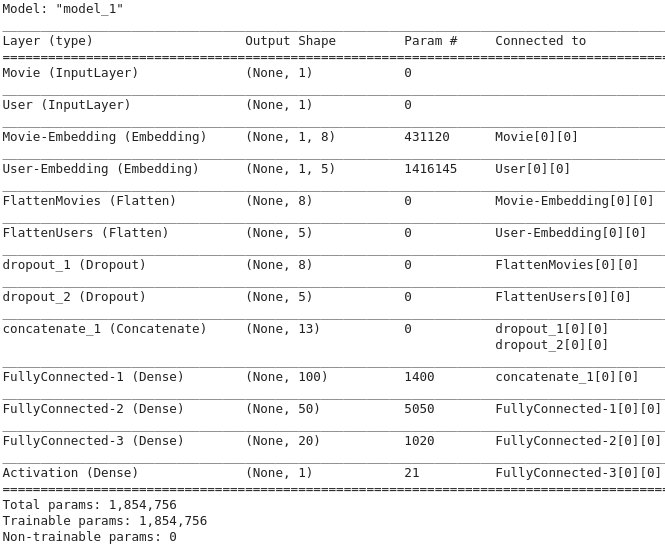
\includegraphics[width=0.5\textwidth]{latex_template/NeuralNetArch.png}

Content Based: The content-based recommendation approach recommends movies to the users according to their preferences and tastes by considering the user's profile. In our approach, we used a list of genres for a movie as content. We created features and vectorized each movie using TF-IDF. Next, we find cosine similarity between movies the user has rated and movies we need to be recommended. For predicting rating for the movie i (movie\_i), we computed the weighted average rating with all the movies that the user has rated(movie\_u) and have positive cosine similarity with movie\_i. Where weight corresponds to cosine similarity between movie\_u and movie\_i. As we are only considering the positive cosine similarity while calculating the weighted average, if there is no movie in movie\_u with positive cosine similarity for movie\_i, then we just take mean of movie\_u as the rating for movie\_i.

SVD: Singular Value Decomposition (SVD)is a matrix decomposition technique which can be used for dimentionality reduction, noise reduction and also compression. SVD is more popular because any real matrix can be decomposed making this technique more stable than even eigen decomposition. In this procedure a real matrix is decomposed into three matrices, say U, Sigma, V{\textsuperscript{T}}, where U and V are composed of orthonormal columns and Sigma is a diagonal matrix with singular values, which help us deduce the most significant correlated properties.

NMF: Non-negative Matrix Factorization (NMF)\cite{nmfwiki} is a dimensionality reduction technique based on decomposition by parts. It takes the n x m utility matrix V with non-negative ratings, where n = total number of users and m = total number of movies, and decomposes it into two non-negative matrices W (n x k) and H (k x m). This is done by solving the optimization problem, \beginmath{} \minimize {\|V - WH\|} \endmath{} such that W\beginmath{}{\geq}\endmath{}0 and H\beginmath{}{\geq}\endmath{}0. A method to solve this optimization using Gradient Descent with Multiplicative Update is discussed in \cite{NIPS2000_1861}.

NMF has an inherent clustering property\cite{Ding05onthe}, it automatically clusters the columns of input matrix V. Furthermore, the computed matrix H gives the cluster membership, i.e., if H \textsubscript{kj} \beginmath{}{\geq}\endmath{} H \textsubscript{ij} for all i ≠ k, this suggests that the input data v \textsubscript{j} belongs to k \textsuperscript{th} cluster. The matrix W gives the cluster centroids, i.e., the k \textsuperscript{th} column gives the cluster centroid of k \textsuperscript{th} cluster. NMF therefore, discovers latent factors in the utility matrix and maps each movie and each user to a k-dimensional concept space.

SlopeOne: Slope One for collaborative filtering was developed by Lemire and Maclachlan\cite{lemire2007slope}. Linear regression f(x)=ax+b can be used to predict the ratings on one item based on the ratings on another item \cite{articleregcoll}. However, severe overfitting issues may arise in this method if pairs of items are selected such that few users have rated both.

\cite{slopeonewiki}A better alternative is using a simpler predictor such as f(x)=x+b (called Slope One), that is experimentally found to give better performance than linear regression, with smaller number of regressors. The free parameter b is the average difference between the two items' ratings. The modified predictor is also efficient in terms of memory requirements and latency.

KNN with Baseline: K-Nearest Neighbours algorithm \cite{10.2307/2685209} finds the unknown ratings of an item using k of the ratings in its neighbourhood. KNN computes similarity of the given item, with other items with known ratings in its neighbourhood, using the Centered Cosine Distance (Pearson Correlation) metric. KNN with baseline \cite{knnbaseline} also includes a base rating for each user-item pair besides the similarity metric. Including baseline estimate models the biases in the prediction thus enhancing the accuracy and reliability of the predictions obtained.

CoClustering: Co clustering or biclustering \cite{RePEc:eee:csdana:v:52:y:2008:i:6:p:3233-3245} allows simultaneous clustering along the rows and columns of the utility matrix. Users and items are assigned to some clusters C\textsubscript{u}, C\textsubscript{i}, and also some co-clusters C\textsubscript{ui}\cite{coclustering}.

\beginmath{}
r_{ui} = \overline{C_{ui}} + (\mu_u - \overline{C_u}) + (\mu_i
- \overline{C_i})
\endmath{}

where \beginmath{}\overline{C_ui}\endmath{} is the average rating of co-cluster C\textsubscript{ui}, \beginmath{}\overline{C_u}\endmath{} is the average rating of u’s cluster, and \beginmath{}\overline{C_i}\endmath{} is the average rating of i’s cluster. If the user is unknown, the prediction is \beginmath{}r^ui=μi\endmath{}. If the item is unknown, the prediction is \beginmath{}r^ui=μu\endmath{}. If both the user and the item are unknown, the prediction is \beginmath{}r^ui=μ\endmath{}.

The clustering itself is done through optimization techniques such as k-means.

ALS: Alternating Least Squares(ALS) is also a matrix factorization algorithm. It is simple and solves scalability and sparseness of the ratings data. ALS runs in a parallel way, minimizing two loss functions alternatively. It first fixes the user matrix and runs gradient descent with item matrix, then it fixes the item matrix and runs gradient descent with user matrix. This way it is useful for larges-scale collaborative filtering problems\cite{als}. 

\section{Experiments}\label{sec:experiments}
The table \ref{tab:Experiment results 1M} presents metrics computed for various individual models as well the ensemble when trained and tested for the 1M MovieLens dataset of approximately 1 million records.

Table \ref{tab:Experiment results 27M} shows the metrics obtained when the models were scaled for the Full Latest MovieLens dataset of approximately 27 million records. Due to computing power limitation and high space complexity of some algorithms presented for 1M, only few of those models were included for analysis on 27 million rating dataset.




Because of large size of dataset most of model was not difficult to train on our local machine. We used google colab platform for the training our algorithms.We ran our neural network model for 15 epochs. we build our model with Keras(Tensorflow backend). For training neural network we used adam optimizer and mean absolute error as loss function. For training ALS we used pyspark's MLLib library of iteration as 20 and for training SVD, KNN, Slopeone, Coclustering, NMF we used surprise library.




\begin{table}
   \caption{Experiment results on 1 Million dataset}\label{tab:Experiment results 1M}
   \small
   \begin{tabular}{|l|c|c|c|c|c|c|}
   \hline
   method&RMSE&MAE&Precision&Recall&FMeasure \\
   \hline\hline
   NeuralNet&0.95&0.71&0.67&0.67&0.67\\
   \hline
   contentBased&0.94&0.71&0.66&0.66&0.66\\
   \hline
   SVD&0.87&0.68&0.68&0.68&0.68\\
   \hline
   NMF&0.91&0.72&0.66&0.66&0.66\\
   \hline
   CoClustering&0.91&0.71&0.67&0.67&0.67\\
   \hline
   ALS&1.25&1.16&0.62&0.62&0.62\\
   \hline
   KNN&0.89&0.70&0.67&0.67&0.67\\
   \hline
   Ensemble&0.87&0.68&0.68&0.68&0.68\\
   \hline
   \end{tabular}
\end{table}

\begin{table}
   \caption{Experiment results on 27 Million data}\label{tab:Experiment results 27M}
   \small 
   \begin{tabular}{|l|c|c|c|c|c|c|}
   \hline
   method&RMSE&MAE&Precision&Recall&FMeasure \\
   \hline\hline
   NeuralNet&0.90&0.66&0.83&0.83&0.83\\
   \hline
   SVD&0.78&0.59&0.85&0.85&0.85\\
   \hline
   NMF&0.87&0.67&0.82&0.82&0.82\\
   \hline
   CoClustering&0.89&0.69&0.83&0.83&0.83\\
   \hline
   ALS&1.29&1.01&0.77&0.77&0.77\\
   \hline
   Ensemble&0.80&0.61&0.84&0.84&0.84\\
   \hline
   \end{tabular}
\end{table}



\section{Conclusions and Future Work}\label{sec:conclusions}
We can see for 1M moivelens dataset, we got best evaluation metrics results by taking ensemble of the all the individual model. For 27M movielens dataset though our evaluation metrics is not better than SVM but after Ensemble Rating outperform all the other method except SVM.

In conclusion, ensemble techniques balanced the bias variance trade-off in ensemble learning and provide better result then base learner.

In future work, we can improve our model by using weighted average of the rating rather than taking simple average. Our result might improve more if we incorporate learning to rank based approached in base model.

\bibliographystyle{ACM-Reference-Format}
\balance
\bibliography{paper}

\end{document}






